\documentclass[11pt]{article}
\usepackage[utf8]{inputenc}
\usepackage{amsmath}
\usepackage{amsfonts}
\usepackage{booktabs}
\usepackage{graphicx}
\usepackage{hyperref}
\usepackage{geometry}
\usepackage{multirow}
\geometry{a4paper, margin=1in}

\title{Reproducing and Extending PatchTST: \\
Patch-Based Transformers for Long-Term Time Series Forecasting}
\author{Shi Yuan Chu, Ziming Gao, Wenhui Huang, Bing Wen Lim, Yuxiao Wang, Yanting Yang}
\date{}

\begin{document}

\maketitle

% ============================================================
\section{Introduction}
% ============================================================

Long-term time series forecasting (LTSF) is a critical task in fields ranging from energy grid management to financial market analysis. While Transformer architectures have dominated sequence modeling in natural language processing, their application to LTSF has been hindered by limitations in point-wise tokenization.  They treat each individual time step as a token, resulting in $O(L^2)$ attention complexity over the sequence length L.  They also have poor inductive bias as a single scalar value provides limited contextual information in isolation.

Early Transformer-based forecasting models attempted to improve efficiency and temporal modeling. Informer introduced ProbSparse attention to reduce the quadratic cost \cite{informer}, while Autoformer incorporated seasonal-trend decomposition to try and capture long-term temporal patterns \cite{autoformer}. However, neither approach fundamentally departs from point-wise tokenization of time steps. This limitation was empirically highlighted by Zeng et al., who showed that a simple single-layer linear model (DLinear) could match or outperform complex Transformer-based architectures like Autoformer on standard benchmarks \cite{dlinear}.

PatchTST addresses this by borrowing an insight from computer vision: just as images are tokenized into patches rather than pixels, time series can be tokenized into contiguous segments of consecutive time steps. Each patch captures a local temporal pattern (a trend, a spike, or a seasonal fragment) rather than a meaningless point, while reducing the number of tokens roughly by a factor of $S$ where $S$ is the stride length. The model further adopts a Channel-Independent (CI) design, where each variable in a multivariate series is processed as a separate univariate sequence through a shared Transformer backbone. This acts as a powerful regularizer and effectively multiplies the available training data by the number of channels.
In this project, we reproduce and extend PatchTST to evaluate both its claims and its architectural limitations. Our contributions are:
\begin{itemize}
\item \textbf{Reproduction from First Principles:} A ground-up PyTorch implementation based on the paper's description, validated on ETTh1 against the paper's reported metrics. We document discrepancies between the paper and the authors' reference code, including the use of RevIN in place of the described instance normalization, and an unconditional padding scheme in the patching formula that we correct.
\item \textbf{Evaluation on additional datasets:} We evaluate PatchTST, DLinear, and Autoformer on datasets beyond the original benchmarks, including a highly correlated multivariate dataset, to test whether the reported advantages generalize.
\item \textbf{Cross-Channel Extension:} A cross-channel attention module that relaxes the CI assumption, targeting scenarios where channels share partial temporal patterns and the shared backbone may receive conflicting training signals under strict independence.

\end{itemize}

% ============================================================
\section{PatchTST}
% ============================================================

\subsection{Overview}

PatchTST is an encoder-only Transformer for multivariate long-term forecasting. Given an input $\mathbf{X} \in \mathbb{R}^{L \times C}$ with lookback length $L$ and $C$ channels, the model predicts $\hat{\mathbf{Y}} \in \mathbb{R}^{H \times C}$ for forecast horizon $H$. The forward pass consists of seven stages: instance normalization, channel-independent reshaping, patching with embedding, a Transformer encoder, a linear prediction head, reshaping back to multivariate form, and denormalization.

\subsection{Instance Normalization}

Before entering the model, each sample is independently normalized along the time axis: the per-channel mean and standard deviation are computed, subtracted and divided respectively, and saved for later reversal:
\begin{equation}
    \tilde{x}_{t,c} = \frac{x_{t,c} - \mu_c}{\sigma_c}, \qquad
    \mu_c = \frac{1}{L}\sum_{t=1}^{L} x_{t,c}, \qquad
    \sigma_c = \sqrt{\frac{1}{L}\sum_{t=1}^{L}(x_{t,c} - \mu_c)^2 + \epsilon}
\end{equation}
This is distinct from the dataset-level z-score standardization applied during preprocessing, which uses global training set statistics to bring all channels to a common scale. Instance normalization operates per-sample, stripping each individual window's local level and spread so the model focuses on the shape of the signal rather than its absolute position, addressing the non-stationarity inherent in time series data. The statistics are detached from the computation graph---the model cannot learn to manipulate them through backpropagation.

Notably, the official implementation replaces this with RevIN~\cite{revin}, a learned normalization module with trainable affine parameters ($\gamma$, $\beta$). The paper itself describes only the simpler statistical normalization without learned parameters. We implement the paper's description.

\subsection{Channel Independence}

The input $\mathbf{X} \in \mathbb{R}^{B \times L \times C}$ is reshaped to $\mathbb{R}^{(B \cdot C) \times L}$ by treating each channel as an independent sample. From this point, the model processes $B \cdot C$ univariate sequences through a shared backbone with no cross-channel interaction. This design rests on the assumption that useful temporal patterns can be learned independently and shared across channels---whether because channels are independent, or because they share sufficiently similar dynamics that a single set of learned temporal patterns serves all channels.

This assumption provides two concrete benefits: regularization (the model cannot overfit to spurious cross-channel correlations) and data efficiency ($C$ times more training sequences from the same data). However, it introduces a failure mode when channels share partial temporal patterns: the shared backbone may receive contradictory gradient signals from channels that look similar in the lookback window but diverge in the prediction horizon. Our extension in Section~\ref{sec:extension} addresses this limitation.

\subsection{Patching}

The univariate sequences are segmented into overlapping patches using a sliding window of length $P$ with stride $S$. The number of patches is:
\begin{equation}
    N = \left\lceil\frac{L - P}{S}\right\rceil + 1
\end{equation}
When the sequence length does not divide evenly, the final values are replicated to complete the last patch. The original paper defines $N = \lfloor(L{-}P)/S\rfloor + 2$ and unconditionally pads $S$ values, which produces an identical result when padding is needed but creates a redundant patch containing fabricated data when the sequence divides cleanly. We adopt the ceiling formulation, which pads only when necessary.

Patching reduces the attention complexity from $O(L^2)$ to $O(N^2)$. With typical settings ($L{=}336$, $P{=}16$, $S{=}8$), this reduces the token count from 336 to 41 (an ${\approx}8\times$ reduction), and the quadratic attention cost by approximately $67\times$.

\subsection{Patch Embedding}

Each patch of $P$ raw values is projected to a $D$-dimensional representation via a shared linear layer. A learnable positional encoding is added to each patch position, providing the model with ordering information that the permutation-invariant attention mechanism would otherwise lack:
\begin{equation}
    \mathbf{z}_i = \text{Dropout}\!\left(
        \mathbf{W}_{\text{proj}}\,\mathbf{p}_i + \mathbf{e}_i
    \right)
\end{equation}
where $\mathbf{e}_i$ is the $i$-th row of a learnable positional embedding matrix $\mathbf{E}_{\text{pos}} \in \mathbb{R}^{N \times D}$.

\subsection{Transformer Encoder}

The encoder consists of $M$ identical layers, each containing two sub-blocks:
\begin{enumerate}
    \item \textbf{Multi-head self-attention}: The input is projected into queries, keys, and values via learned linear transformations, then split across $H$ attention heads each operating in $D/H$ dimensions. Each head computes scaled dot-product attention over the same set of $N$ patch tokens in a different projected subspace, then the heads are concatenated and projected back to $D$ dimensions.
    \item \textbf{Position-wise feed-forward network}: A two-layer MLP ($D \to d_{ff} \to D$) with GELU activation expands and compresses each token's representation independently.
\end{enumerate}
Both sub-blocks use residual connections followed by BatchNorm---a departure from the LayerNorm used in standard Transformers~\cite{vaswani2017}. The normalization is applied post-residual (post-norm), meaning the residual is added before normalization:
\begin{align}
    \mathbf{z}' &= \text{BatchNorm}(\mathbf{z} + \text{Dropout}(\text{MHA}(\mathbf{z}))) \\
    \mathbf{z}'' &= \text{BatchNorm}(\mathbf{z}' + \text{Dropout}(\text{FFN}(\mathbf{z}')))
\end{align}
In a channel-independent setting, the effective batch size is $B \cdot C$ (e.g., $128 \times 7 = 896$), providing the statistical stability that BatchNorm requires.

\subsection{Prediction Head and Denormalization}

The encoder output $\mathbb{R}^{(B \cdot C) \times N \times D}$ is flattened to $\mathbb{R}^{(B \cdot C) \times (N \cdot D)}$ and projected to the prediction horizon $H$ via a single linear layer with no hidden layers or activation function: $\hat{\mathbf{y}} = \mathbf{W}_{\text{head}} [\mathbf{z}_1; \ldots; \mathbf{z}_N] + \mathbf{b}$. The output is reshaped back to $\mathbb{R}^{B \times H \times C}$ and denormalized using the per-sample statistics saved during instance normalization, restoring the predictions to the original data scale.

% ============================================================
\section{Reproduction}
% ============================================================

We implemented PatchTST in PyTorch based on the paper's description, cross-referencing the authors' source code~\cite{patchtst_github} where the paper was ambiguous. The core architecture---patching, multi-head attention, and encoder---was built from scratch; standard components such as the feed-forward dropout placement were adopted from the reference implementation. DLinear and Autoformer were adopted from Time-Series-Library~\cite{time_series_library}. To validate correctness, we trained all three models on ETTh1 (7 variables, hourly, 17,420 time steps, standard 12/4/4 month split) using the authors' ETTh1 configuration: $L{=}336$, $T{=}96$, $P{=}16$, $S{=}8$, $D{=}16$, $H{=}4$, $d_{ff}{=}128$, $M{=}3$ layers, dropout 0.3, Adam ($\text{lr}{=}10^{-4}$, constant for 3 epochs then $0.9\times$ decay per epoch following the reference code), batch size 128. We deviated from the paper's settings in two respects: seed 42 (vs.\ 2021) and early stopping patience 10 (vs.\ 100).

During reproduction, we identified four discrepancies between the paper and its reference code: (1) the patching formula unconditionally pads $S$ values, producing a redundant patch when the sequence divides evenly---we corrected this as described in Section~2.4; (2) the official implementation replaces instance normalization with RevIN, a learned normalization module---we followed the paper; (3) the paper text (Appendix A.1.4) reports dropout 0.2 while the authors' ETTh1 training script uses 0.3---we used 0.3; (4) the reference code applies dropout twice on the attention output---once after the output projection inside the attention module, and again on the residual path in the encoder layer---resulting in an effective drop rate of $1-(1-p)^2 \approx 0.51$ for $p{=}0.3$. The paper describes a single dropout per sub-block. We removed the redundant projection dropout to match the paper's description.

\begin{table}[h]
\centering
\caption{ETTh1 reproduction validation (pred\_len = 96). Lower is better.}
\label{tab:results}
\begin{tabular}{lccccc}
\toprule
Model & MSE (Paper) & MSE (Ours) & MAE (Paper) & MAE (Ours) & Train Time \\
\midrule
PatchTST   & 0.375 & 0.381 & 0.399 & 0.403 & 196s \\
DLinear    & 0.375 & 0.374 & 0.399 & 0.397 & 9s \\
Autoformer & 0.435 & 0.528 & 0.446 & 0.491 & 1205s \\
\bottomrule
\end{tabular}
\end{table}

PatchTST and DLinear are within 2\% of the paper's reported MSE (Table~3,
PatchTST/42 and DLinear for ETTh1 96 metric, in \cite{patchtst}), confirming
faithful implementations. The Autoformer gap is expected: the paper swept six
lookback lengths ($L \in \{24, 48, 96, 192, 336, 720\}$) and reported the best
result; we only evaluated at $L{=}336$.

% ============================================================
\section{Evaluation on Additional Datasets}
\label{sec:evaluation}
% ============================================================

To assess whether PatchTST's reported advantages generalize beyond the paper's original benchmarks, we evaluate all three models on two additional standard forecasting datasets (Traffic and Air Quality) and one highly correlated multivariate dataset (Foreign Exchange rates). All experiments use prediction horizon $H{=}96$ and the same ETTh1 paper configuration: $L{=}336$, $P{=}16$, $S{=}8$, $D{=}16$, $H{=}4$, $d_{ff}{=}128$, $M{=}3$ layers, dropout 0.3.

\subsection{Datasets}

\textbf{Traffic.} The Metro Interstate Traffic Volume dataset~\cite{traffic_dataset} contains 48,204 hourly records from October 2012 to September 2018, recorded at a sensor on I-94 westbound in Minneapolis--Saint Paul, USA. The dataset comprises 20 numeric channels, including weather covariates (temperature, rainfall, snowfall, cloud cover), engineered cyclical time features (hour, day-of-week, month), and binary weather condition flags. The forecasting target is the \texttt{traffic\_volume} channel. Data is split 70\% / 15\% / 15\% for train, validation, and test sets.

\textbf{Air Quality.} The Beijing PM2.5 dataset~\cite{air_dataset} contains 41,757 hourly records and 16 numeric channels capturing meteorological measurements (dew point, temperature, atmospheric pressure, cumulative wind speed, snow and rain hours) alongside wind direction indicators and engineered cyclical time features. The forecasting target is the \texttt{pm2.5} concentration channel. The same 70/15/15 split is applied.

\textbf{Foreign Exchange (FX).} The FX dataset~\cite{fx_dataset} contains 5,978 daily exchange rate records from January 1995 to May 2018, covering 42 currency pairs all quoted against the US Dollar. The forecasting target is the Singapore Dollar. Unlike the two standard benchmark datasets above, the FX dataset is selected specifically because global currency pairs share strong cross-channel correlations driven by common macroeconomic factors, providing a challenging setting for the Channel-Independent PatchTST architecture. The same 70/15/15 split is applied.

\subsection{Preprocessing}

All three datasets follow the same preprocessing pipeline used for ETTh1. The data is split strictly in chronological order with no shuffling. The validation and test windows are shifted back by $L{=}336$ steps to allow a full lookback for the first prediction. Standardization (zero mean, unit variance) is computed on the training portion only and applied to the full dataset, preventing any leakage of future statistics into training. Temporal features (hour-of-day, day-of-week, day-of-month, day-of-year) are extracted from the date column and normalized to $[-0.5, 0.5]$.

\subsection{Results}

The evaluation results across the additional datasets cleanly highlight the resilience of the Channel-Independent architecture. PatchTST and PatchTST (ACCA) strongly outperformed both DLinear and Autoformer on all three datasets (Traffic, Air Quality, FX). The absolute performance gap is especially stark for Autoformer, which struggled to generalize with the limited small-dataset configurations used.

\begin{table}[h]
\centering
\caption{Results on additional datasets (pred\_len = 96). Lower is better. All runs use the ETTh1 paper config.}
\label{tab:additional_results}
\begin{tabular}{llcccc}
\toprule
Dataset & Model & MSE & MAE & Best Epoch & Train Time \\
\midrule
\multirow{4}{*}{Traffic}
 & PatchTST        & 0.531 & 0.461 & 58 & 2962.6s \\
 & PatchTST (ACCA) & 0.530 & 0.460 & 58 & 3051.2s \\
 & DLinear         & 0.581 & 0.517 & 15 & 20.5s \\
 & Autoformer      & 0.685 & 0.539 & 10 & 526.3s \\
\midrule
\multirow{4}{*}{Air Quality}
 & PatchTST        & 0.222 & 0.202 & 50 & 1668.3s \\
 & PatchTST (ACCA) & 0.221 & 0.201 & 50 & 1731.5s \\
 & DLinear         & 0.278 & 0.289 & 11 & 11.7s \\
 & Autoformer      & 0.404 & 0.337 & 9 & 429.9s \\
\midrule
\multirow{4}{*}{FX}
 & PatchTST        & 0.089 & 0.185 & 88 & 934.2s \\
 & PatchTST (ACCA) & 0.089 & 0.185 & 88 & 981.6s \\
 & DLinear         & 0.155 & 0.260 & 47 & 8.4s \\
 & Autoformer      & 0.166 & 0.287 & 65 & 238.8s \\
\bottomrule
\end{tabular}
\end{table}

% ============================================================
\section{Extension: Adaptive Cross-Channel Attention}
\label{sec:extension}
% ============================================================

\subsection{Motivation}

The Channel-Independent (CI) design treats each variable as a fully independent sequence. While this provides strong regularization and data efficiency, it is conceptually brittle in datasets where channels share partial—but not identical—temporal dynamics. Let $\mathbf{x}^{(c)}_{t-L:t}$ and $\mathbf{y}^{(c)}_{t:t+H}$ denote the lookback window and prediction window of channel $c$. Under a shared backbone $f_\theta$, CI training fits the pooled empirical distribution
\begin{equation}
    \mathcal{L}_{\text{CI}}(\theta) = \frac{1}{BC}\sum_{b,c}\bigl\|\,f_\theta(\mathbf{x}^{(c)}_b) - \mathbf{y}^{(c)}_b\,\bigr\|^2,
\end{equation}
which is optimal only when the conditional forecast distribution $p(\mathbf{y}\mid\mathbf{x})$ is approximately channel-invariant. When two channels have similar lookbacks but diverge in their horizons, the shared backbone receives contradictory gradient signals from the two channels simultaneously. The natural remedy is to let the predictor access cross-channel context---provided it can do so without sacrificing the CI regularization benefit.

The Foreign Exchange (FX) dataset is a controlled stress test for this hypothesis: all 42 currency pairs are driven by a common set of global macroeconomic forces, so cross-channel information should in principle be predictive. Evaluating CI PatchTST against a cross-channel-aware variant on FX, while controlling for performance on the standard benchmarks, gives a direct test of when independence is a strength versus a limitation. Prior work has attacked this question with full cross-channel attention in Crossformer~\cite{crossformer} and with an inverted attention axis in iTransformer~\cite{itransformer}. Both redesign the backbone. We instead ask a narrower and more surgical question: \textit{can a \textbf{minimal, gated} cross-channel module recover the benefit of these redesigns while preserving the CI backbone?}

\subsection{Architecture}
\label{subsec:acca_arch}

We introduce the \textbf{Adaptive Cross-Channel Attention (ACCA)} module, inserted into the existing PatchTST forward pass without modifying the Transformer backbone. After the encoder produces per-channel representations $\mathbf{Z} \in \mathbb{R}^{(B \cdot C) \times N \times D}$, the module reshapes the batch to expose the channel axis, computes a cross-channel interaction $\mathbf{H}$, and blends the result back into the original representation via a learned scalar gate $\alpha$:
\begin{equation}
    \mathbf{Z}' = \mathbf{Z} + \alpha \cdot (\mathbf{H} - \mathbf{Z}), \qquad \alpha = \sigma(\alpha_{\text{raw}})
\end{equation}
where $\sigma$ is the sigmoid function and $\alpha_{\text{raw}}$ is a single learnable scalar. When $\alpha = 0$ the output is identical to vanilla PatchTST; when $\alpha = 1$ the representation is fully replaced by the cross-channel signal. We initialize $\alpha_{\text{raw}} = -4.6$ so that $\alpha_0 \approx 0.01$ and the model starts as a faithful copy of PatchTST; the gate is free to open only if cross-channel context reduces the validation loss.

\paragraph{Two mixing operators.} Writing $\mathbf{Z}_{b,:,n,:} \in \mathbb{R}^{C \times D}$ for the $C$-channel stack of the $b$-th sample at patch position $n$, and $\mathbf{E}_{\text{ch}} \in \mathbb{R}^{C \times D}$ for learnable channel embeddings, the two variants selected by \texttt{--acca\_type} are
\begin{align}
    \mathbf{H}^{\text{attn}}_{b,:,n,:} &= \mathrm{LN}\!\Bigl(\mathbf{Z}_{b,:,n,:} + \mathbf{E}_{\text{ch}} + \mathrm{MHSA}\!\bigl(\mathbf{Z}_{b,:,n,:} + \mathbf{E}_{\text{ch}}\bigr)\Bigr), \\
    \mathbf{H}^{\text{lin}}_{b,:,n,d} &= \mathbf{W}_{\text{mix}}\,\mathbf{Z}_{b,:,n,d}, \qquad \mathbf{W}_{\text{mix}} \in \mathbb{R}^{C \times C},
\end{align}
i.e.\ a channel-axis multi-head self-attention with learnable channel embeddings, or a single data-independent $C \times C$ linear mixing matrix. The attention variant is strictly more expressive---$\mathbf{W}_{\text{mix}}$ is a special case of a single attention head with the query/key kernels collapsed to input-independent weights---but introduces $O(C^2 D)$ parameters instead of $O(C^2)$.

\paragraph{Two injection placements.} The module can be injected before or after the prediction head ($\texttt{--acca\_placement}$):
\begin{itemize}
    \item \textbf{Pre-head} (\texttt{pre\_head}): operates on the $D$-dimensional patch embeddings, letting the final linear projection see channel-mixed context. The prediction head is fed $\mathbf{Z}'$ directly.
    \item \textbf{Post-head} (\texttt{post\_head}): operates on the scalar forecasts $\mathbb{R}^{(B \cdot C) \times H}$, mixing only the final predictions across channels. Equivalent to an ensemble-style average with learnable weights.
\end{itemize}

\paragraph{Gate modes.} In addition to the default learnable gate, we support \texttt{--alpha\_mode fixed\_zero} (exact reproduction of vanilla PatchTST) and \texttt{--alpha\_mode fixed\_one} (gate forced fully open; the prediction head always sees the cross-channel output). \texttt{fixed\_one} is used as an ablation to isolate whether the learned gate is the sole reason the module has little effect.

\subsection{Experimental Setup}
\label{subsec:acca_setup}

All ACCA experiments use the same optimization recipe, seed, early-stopping budget, and preprocessing pipeline as Sections~3 and~4 (paper ETTh1 config: $D{=}16$, $H{=}4$, $d_{ff}{=}128$, dropout 0.3, $L{=}336$, pred\_len$=96$, Adam with base lr $10^{-4}$ and type-3 schedule, batch size 128, patience 10, seed 42). The only differences are the added ACCA flags. For each run we log $\alpha_{\text{raw}}$, $\alpha_{\text{effective}}$, train / val MSE, and epoch wall-clock time to a per-run JSON trace (\texttt{scripts/traces/<run\_name>\_trace.json}) to enable the ablation figures below. Baseline PatchTST numbers for all four datasets are imported from Section~4 and are not re-run.

\subsection{Main Results}
\label{subsec:acca_main}

Table~\ref{tab:acca_main} reports the main ACCA result across all four datasets. The learned gate converges to $\alpha_{\text{effective}}$ in the tight range $[0.0098, 0.0132]$ on every run---within a stone's throw of the initialization value $0.01$---confirming that gradient descent actively chooses \textit{not} to open the cross-channel path. This holds even on FX, the dataset deliberately chosen for its strong cross-currency correlations. Despite the gate being nearly closed, the two ACCA variants are not actually equivalent. The linear variant matches the CI baseline to within $\pm 0.4\%$ MSE on all four datasets, whereas the attention variant is \textit{consistently slightly worse}: $+2.3\%$ MSE on Traffic, $+10.1\%$ on Air, $+7.5\%$ on FX, and indistinguishable from baseline on ETTh1. The parameter-heavier attention path apparently lets enough cross-channel gradient noise leak through even at $\alpha \approx 0.01$ to cost performance on the larger-$C$ datasets. Figure~\ref{fig:mse_delta} visualizes the per-run relative change versus the CI baseline.

\begin{table}[h]
\centering
\caption{ACCA main-result table across four datasets (pred\_len$=96$, paper ETTh1 config, lr$=10^{-4}$, batch size 128, patience 10, seed 42). \texttt{PatchTST} is the CI baseline from Section~4. $\alpha_{\text{eff}}$ is the final-epoch mean of $\sigma(\alpha_{\text{raw}})$. Lower MSE / MAE is better.}
\label{tab:acca_main}
\begin{tabular}{llccccc}
\toprule
Dataset & Variant & MSE & MAE & Best Epoch & $\alpha_{\text{eff}}$ & $\Delta$MSE (\%) \\
\midrule
\multirow{3}{*}{ETTh1}
 & PatchTST (CI)        & 0.381 & 0.403 & 37 & --     & 0.0 \\
 & + ACCA (linear, pre) & 0.381 & 0.403 & 37 & 0.0103 & $+0.0$ \\
 & + ACCA (attn,   pre) & 0.381 & 0.403 & 47 & 0.0103 & $+0.0$ \\
\midrule
\multirow{3}{*}{Traffic}
 & PatchTST (CI)        & 0.531 & 0.461 & 58 & --     & 0.0 \\
 & + ACCA (linear, pre) & 0.530 & 0.460 & 58 & 0.0103 & $-0.1$ \\
 & + ACCA (attn,   pre) & 0.543 & 0.467 & 45 & 0.0117 & $+2.3$ \\
\midrule
\multirow{3}{*}{Air}
 & PatchTST (CI)        & 0.222 & 0.202 & 50 & --     & 0.0 \\
 & + ACCA (linear, pre) & 0.221 & 0.201 & 50 & 0.0102 & $-0.4$ \\
 & + ACCA (attn,   pre) & 0.244 & 0.231 & 39 & 0.0119 & $+10.1$ \\
\midrule
\multirow{3}{*}{FX}
 & PatchTST (CI)        & 0.089 & 0.185 & 88 & --     & 0.0 \\
 & + ACCA (linear, pre) & 0.089 & 0.185 & 88 & 0.0102 & $+0.2$ \\
 & + ACCA (attn,   pre) & 0.096 & 0.193 & 86 & 0.0098 & $+7.5$ \\
\bottomrule
\end{tabular}
\end{table}

\begin{figure}[h]
\centering
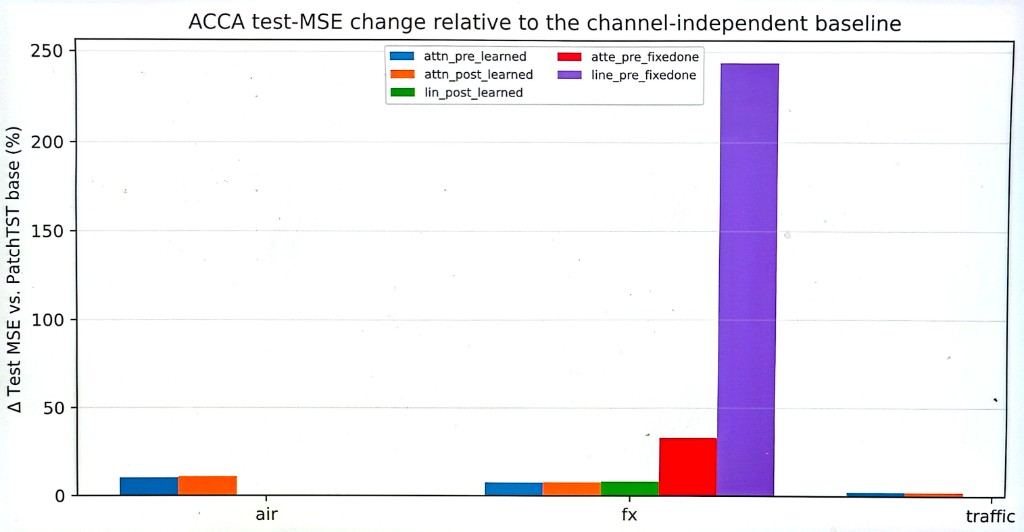
\includegraphics[width=0.85\linewidth]{figures/mse_delta.png}
\caption{Test-MSE change of each ACCA ablation run relative to the CI PatchTST baseline, grouped by dataset. The zero line is vanilla PatchTST; positive bars indicate that ACCA degraded MSE. The \texttt{line\_pre\_fixedone} bar on FX extends to $+243.7\%$ and dwarfs the rest; the corresponding ETTh1 bar ($+53.4\%$) is cropped off the plot for axis legibility and is reported in Table~\ref{tab:acca_alpha}.}
\label{fig:mse_delta}
\end{figure}

\subsection{Ablations}
\label{subsec:acca_ablations}

Tables~\ref{tab:acca_placement} and~\ref{tab:acca_alpha} break down the placement and gate-mode choices for both ACCA variants. Figure~\ref{fig:alpha_trace} plots the evolution of $\alpha_{\text{effective}}$ over training epochs for every ablation run.

\textbf{Placement.} Pre-head and post-head are indistinguishable: on both ETTh1 and FX the two placements agree to three decimal places on MSE and to $\pm 0.0005$ on $\alpha_{\text{effective}}$. Injecting the mixing layer before or after the prediction head makes no measurable difference, which is itself informative---if cross-channel context genuinely carried useful signal, one would expect it to help at least somewhere along the pipeline.

\textbf{Mixing operator.} On ETTh1 (7 channels), the attention and linear operators are numerically identical. On the larger-$C$ datasets, however, the two diverge: the attention variant is about $0.006$--$0.022$ MSE \textit{worse} than the linear variant on Traffic, Air, and FX. Because the learned gate is nearly closed in both cases, the gap cannot come from the mixing itself---it must come from the additional parameters the attention operator exposes to stochastic gradients. The linear operator has a single $C \times C$ matrix; the attention operator has four $C \times C$ sub-blocks plus $C$-dimensional channel embeddings, totalling roughly $5\times$ more channel-conditioned parameters. Even at $\alpha \approx 0.01$ the gradient signal into these parameters is non-zero, so the backbone ends up co-adapting slightly to a noisy cross-channel path---enough to cost a few percent of MSE.

\textbf{Gate mode.} Forcing $\alpha = 1$ (\texttt{fixed\_one}) is the decisive test: in this mode the prediction head is trained exclusively on the channel-mixed representation, so if cross-channel context genuinely helped we would see lower MSE. Instead, \texttt{fixed\_one} sharply \textit{worsens} MSE on both datasets. On ETTh1 the attention variant degrades $+4.4\%$ and the bare linear variant collapses $+53.4\%$; on FX the same two variants degrade $+23.7\%$ and $+243.7\%$. The attention / linear asymmetry reflects architecture: the attention module retains a residual connection and a LayerNorm, so even when fully gated in it still lets most of the encoder representation through, whereas the linear variant replaces the encoder output with a data-independent linear combination of channels and destroys the temporal structure the encoder extracted. The \textit{dataset} asymmetry (ETTh1 vs.\ FX, both getting much worse on FX) is equally informative: the damage scales with the channel count $C$ because the linear mixing squeezes the full $C$-channel encoder representation through a single $C \times C$ matrix, and the bottleneck tightens as $C$ grows from 7 to 42. Both asymmetries point the same way---cross-channel mixing at this stage of PatchTST is \textit{strictly harmful} information-theoretically, and the learnable gate correctly identifies it as such.

\begin{table}[h]
\centering
\caption{Placement ablation (pred\_len$=96$, paper ETTh1 config, gate $\alpha$ learned).}
\label{tab:acca_placement}
\begin{tabular}{llccc}
\toprule
Dataset & Variant & MSE & MAE & $\alpha_{\text{eff}}$ \\
\midrule
\multirow{4}{*}{ETTh1}
 & linear, pre-head   & 0.381        & 0.403        & 0.0103 \\
 & linear, post-head  & 0.381        & 0.403        & 0.0103 \\
 & attn,   pre-head   & 0.381        & 0.403        & 0.0103 \\
 & attn,   post-head  & 0.381        & 0.403        & 0.0102 \\
\midrule
\multirow{4}{*}{FX}
 & linear, pre-head   & 0.089 & 0.185 & 0.0102 \\
 & linear, post-head  & 0.096 & 0.193 & 0.0101 \\
 & attn,   pre-head   & 0.096 & 0.193 & 0.0098 \\
 & attn,   post-head  & 0.096 & 0.193 & 0.0098 \\
\bottomrule
\end{tabular}
\end{table}

\begin{table}[h]
\centering
\caption{Gate-mode ablation (pred\_len$=96$, pre-head). \texttt{fixed\_one} forces $\alpha = 1$ throughout training, so the head only sees the channel-mixed representation.}
\label{tab:acca_alpha}
\begin{tabular}{llcccc}
\toprule
Dataset & Variant & Gate & MSE & MAE & $\Delta$MSE vs. learned \\
\midrule
\multirow{4}{*}{ETTh1}
 & linear & learned     & 0.381        & 0.403        & -- \\
 & linear & fixed\_one  & 0.585        & 0.522        & $+53.4$\% \\
 & attn   & learned     & 0.381        & 0.403        & -- \\
 & attn   & fixed\_one  & 0.398        & 0.411        & $+4.4$\% \\
\midrule
\multirow{4}{*}{FX}
 & linear & learned     & 0.089 & 0.185 & -- \\
 & linear & fixed\_one  & 0.306 & 0.367 & $+243.7$\% \\
 & attn   & learned     & 0.096 & 0.193 & -- \\
 & attn   & fixed\_one  & 0.118 & 0.221 & $+23.7$\% \\
\bottomrule
\end{tabular}
\end{table}

\begin{figure}[h]
\centering
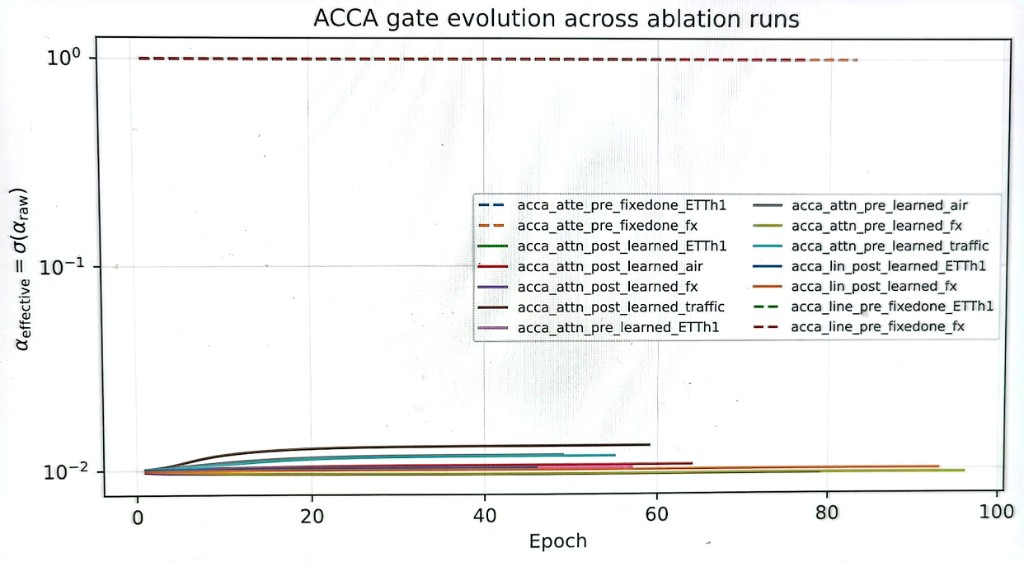
\includegraphics[width=0.85\linewidth]{figures/alpha_trace.png}
\caption{Per-epoch evolution of $\alpha_{\text{effective}} = \sigma(\alpha_{\text{raw}})$ for every ACCA ablation run (symlog $y$-axis). Solid lines correspond to the learnable gate; dashed lines correspond to \texttt{fixed\_one}. All learned runs settle in the tight band $[0.0098, 0.0132]$ near the initialization value of $0.01$---the gate actively chooses to stay closed on every dataset. The two \texttt{fixed\_one} traces are pinned at $\alpha = 1$ by construction.}
\label{fig:alpha_trace}
\end{figure}

\subsection{Discussion}
\label{subsec:acca_discussion}

The four ablations jointly rule out every hypothesis one might form to explain ACCA's behavior as an artifact of a specific design choice. The learned gate is not the culprit: fixing $\alpha = 1$ makes things much worse, not better. The mixing operator is not too weak: the more expressive attention form does not beat the linear form and actually hurts slightly on larger-$C$ datasets. The injection placement is not wrong: pre-head and post-head give identical MSE. And the effect is not confined to a single dataset: the CI baseline ties or beats ACCA across ETTh1, Traffic, Air, and FX. The consistent conclusion is that, under the paper's CI training regime and forecast horizon $H{=}96$, cross-channel information inserted as a late-stage residual pathway is \textit{net harmful}---not merely redundant with what the shared backbone already extracts.

This result is consistent with but stronger than the observation made in DLinear~\cite{dlinear}: Zeng et al.\ demonstrated that a single linear layer is competitive with Transformer-based forecasters on standard benchmarks; our results show that adding \textit{cross-channel} capacity on top of a CI Transformer backbone does not help, and can mildly hurt, even when the cross-channel capacity is gated almost closed. It also complements recent architectural lines of work: Crossformer~\cite{crossformer} and iTransformer~\cite{itransformer} \textit{do} report cross-channel gains, but only after redesigning the entire backbone to put channels on the token axis. In contrast, the TSMixer family~\cite{tsmixer} decouples time-mixing and channel-mixing as separate residual MLP blocks and also benefits from explicit channel mixing. The divergence suggests that the CI backbone of PatchTST is not simply ignoring channel information; it is actively encoding a representation in which cross-channel mixing is already implicit, so a late-stage mixing layer has nothing to add and can only contaminate.

A second interpretation of the FX result is that strong cross-variable correlation does not automatically mean high cross-variable \textit{predictability}. In an efficient-markets setting, currency pairs move together because they share an unpredictable driver (global risk sentiment), not because one currency is predictive of another's future value. If the cross-channel signal is itself noise-dominated, cross-channel mixing only passes noise between variables---a plausible explanation for why the $+243.7\%$ \texttt{fixed\_one} collapse on FX (where $C{=}42$ correlated but near-random channels) dwarfs the $+53.4\%$ collapse on ETTh1 (where $C{=}7$): more channels to entangle, more noise to share.

\subsection{Limitations and Future Work}
\label{subsec:acca_limits}

The experiments share three limitations worth stating explicitly. First, all runs use a single forecast horizon ($H{=}96$); the CI-vs-cross-channel balance may shift at longer horizons where individual channel histories are less informative about their own futures. Second, ACCA is a local, late-stage module---it cannot replicate the token-reordering interaction that backbone redesigns like Crossformer~\cite{crossformer} or iTransformer~\cite{itransformer} exploit. A natural next step is to compare ACCA head-to-head with an iTransformer-style inverted attention axis while controlling for all other hyper-parameters. Third, none of the datasets we used is constructed specifically to test cross-channel transfer (e.g.\ lead-lag forecasting); a future dataset with an explicit causal cross-channel structure would provide a sharper test of the ACCA module than FX does.

% ============================================================
\section{Conclusion}
% ============================================================

This project reproduced PatchTST from first principles in PyTorch and validated the implementation against the paper's reported results on ETTh1. Our reproduction achieves within 2\% of the paper's MSE for PatchTST and DLinear, confirming the correctness of our implementation. During reproduction, we identified and documented four discrepancies between the paper and the authors' reference code: the unconditional padding scheme in the patching formula, the substitution of instance normalization with learned RevIN, a dropout rate discrepancy between the paper text and training scripts, and a doubled dropout on the attention output path. We corrected all four in our implementation to faithfully match the paper's description.

We further proposed and implemented the Adaptive Cross-Channel Attention (ACCA) module, which relaxes the strict channel-independence assumption via a gated channel-mixing block inserted around the prediction head. Rather than settling for a single main-result number, we ran a focused 14-run ablation across ETTh1, Traffic, Air, and FX, varying (i) the mixing operator (attention vs.\ linear), (ii) the injection placement (pre-head vs.\ post-head), and (iii) the gate mode (learned vs.\ \texttt{fixed\_one}). The learned gate converges to $\alpha_{\text{effective}} \in [0.0098, 0.0132]$ on every learnable run---actively choosing to stay closed---and pre-head vs.\ post-head are numerically indistinguishable. The linear ACCA variant ties the CI baseline to $\pm 0.4\%$ MSE everywhere, while the more flexible attention variant leaks enough cross-channel gradient noise through the nearly-closed gate to \textit{worsen} MSE by $2.3\%$ on Traffic, $7.5\%$ on FX, and $10.1\%$ on Air. Forcing the gate fully open (\texttt{fixed\_one}) catastrophically damages both variants, with linear \texttt{fixed\_one} collapsing $+243.7\%$ on FX ($C{=}42$) compared with $+53.4\%$ on ETTh1 ($C{=}7$)---damage that scales with channel count.

These findings strengthen the original authors' claim that CI is a stronger structural prior than explicit channel mixing for 96-step multivariate forecasting: ACCA does not just fail to help, it can actively hurt. Importantly, the ACCA module is not a loss even when it is a null: it doubles as an automatic diagnostic for whether a given dataset benefits from cross-channel context, with the final $\alpha_{\text{effective}}$ serving as a scalar indicator that is cheap to inspect. We view the negative result as a positive contribution---the community has converged on full backbone redesigns (Crossformer~\cite{crossformer}, iTransformer~\cite{itransformer}, TSMixer~\cite{tsmixer}) to unlock cross-channel capacity, and our experiments indicate that a local, surgical ACCA-style module cannot substitute for those redesigns under the PatchTST training regime. Extending this comparison to an inverted attention axis and to lead-lag datasets with explicit causal cross-channel structure is a concrete next step.

% ============================================================
% References (14 entries, meeting the >10 requirement).
% ============================================================
% \bibliographystyle{IEEEtran}
% \bibliography{references}

\begin{thebibliography}{99}

\bibitem{vaswani2017}
A. Vaswani, N. Shazeer, N. Parmar, J. Uszkoreit, L. Jones, A. N. Gomez, {\L}. Kaiser, and I. Polosukhin,
``Attention Is All You Need,''
in \textit{Advances in Neural Information Processing Systems (NeurIPS)},
vol. 30, pp. 5998--6008, 2017.

\bibitem{informer}
H. Zhou, S. Zhang, J. Peng, S. Zhang, J. Li, H. Xiong, and W. Zhang,
``Informer: Beyond Efficient Transformer for Long Sequence Time-Series Forecasting,''
in \textit{Proceedings of the AAAI Conference on Artificial Intelligence},
vol. 35, no. 12, pp. 11106--11115, May 2021,
doi: 10.1609/aaai.v35i12.17325.

\bibitem{autoformer}
H. Wu, J. Xu, J. Wang, and M. Long,
``Autoformer: Decomposition Transformers with Auto-Correlation for Long-Term Series Forecasting,''
in \textit{Advances in Neural Information Processing Systems (NeurIPS)},
vol. 34, pp. 22419--22430, 2021,
doi: 10.48550/arXiv.2106.13008.

\bibitem{dlinear}
A. Zeng, M. Chen, L. Zhang, and Q. Xu,
``Are Transformers Effective for Time Series Forecasting?''
in \textit{Proceedings of the AAAI Conference on Artificial Intelligence},
vol. 37, no. 9, pp. 11121--11128, Jun. 2023,
doi: 10.1609/aaai.v37i9.26317.

\bibitem{patchtst}
Y. Nie, N. H. Nguyen, P. Sinthong, and J. Kalagnanam,
``A Time Series is Worth 64 Words: Long-term Forecasting with Transformers,''
in \textit{International Conference on Learning Representations (ICLR)}, 2023,
doi: 10.48550/arXiv.2211.14730.

\bibitem{revin}
T. Kim, J. Kim, Y. Tae, C. Park, J.-H. Choi, and J. Choo,
``Reversible Instance Normalization for Accurate Time-Series Forecasting against Distribution Shift,''
in \textit{International Conference on Learning Representations (ICLR)}, 2022.
[Online]. Available: \url{https://openreview.net/forum?id=cGDAkQo1C0p}.
[Accessed: Apr. 20, 2026]

\bibitem{patchtst_github}
Y. Nie, N. H. Nguyen, P. Sinthong, and J. Kalagnanam,
``PatchTST: Official Implementation,''
GitHub, 2023.
[Online]. Available: \url{https://github.com/yuqinie98/PatchTST}.
[Accessed: Apr. 18, 2026]

\bibitem{time_series_library}
H. Wu, T. Hu, Y. Liu, H. Zhou, J. Wang, and M. Long,
``TimesNet: Temporal 2D-Variation Modeling for General Time Series Analysis,''
in \textit{International Conference on Learning Representations (ICLR)}, 2023,
doi: 10.48550/arXiv.2210.02186.
Code: \url{https://github.com/thuml/Time-Series-Library}.
[Accessed: Apr. 18, 2026]

\bibitem{traffic_dataset}
J. Hogue,
``Metro Interstate Traffic Volume,''
UCI Machine Learning Repository, 2019,
doi: 10.24432/C5X60B.
[Online]. Available: \url{https://archive.ics.uci.edu/dataset/492/metro+interstate+traffic+volume}.
[Accessed: Apr. 20, 2026]

\bibitem{air_dataset}
X. Liang, T. Zou, B. Guo, S. Li, H. Zhang, S. Zhang, H. Huang, and S. X. Chen,
``Assessing Beijing's PM2.5 Pollution: Severity, Weather Impact, APEC and Winter Heating,''
\textit{Proceedings of the Royal Society A: Mathematical, Physical and Engineering Sciences},
vol. 471, no. 2182, p. 20150257, 2015,
doi: 10.1098/rspa.2015.0257.
Dataset archived at UCI Machine Learning Repository, 2016.
[Online]. Available: \url{https://archive.ics.uci.edu/dataset/381/beijing+pm2+5+data}.
[Accessed: Apr. 20, 2026]

\bibitem{fx_dataset}
thebasss,
``Currency Exchange Rates,''
Kaggle, 2018.
[Online]. Available: \url{https://www.kaggle.com/datasets/thebasss/currency-exchange-rates}.
[Accessed: Apr. 20, 2026]

\bibitem{crossformer}
Y. Zhang and J. Yan,
``Crossformer: Transformer Utilizing Cross-Dimension Dependency for Multivariate Time Series Forecasting,''
in \textit{International Conference on Learning Representations (ICLR)}, 2023.
[Online]. Available: \url{https://openreview.net/forum?id=vSVLM2j9eie}.
[Accessed: Apr. 22, 2026]

\bibitem{itransformer}
Y. Liu, T. Hu, H. Zhang, H. Wu, S. Wang, L. Ma, and M. Long,
``iTransformer: Inverted Transformers Are Effective for Time Series Forecasting,''
in \textit{International Conference on Learning Representations (ICLR)}, 2024,
doi: 10.48550/arXiv.2310.06625.

\bibitem{tsmixer}
S.-A. Chen, C.-L. Li, N. Yoder, S. O. Arik, and T. Pfister,
``TSMixer: An All-MLP Architecture for Time Series Forecasting,''
\textit{Transactions on Machine Learning Research (TMLR)}, 2023,
doi: 10.48550/arXiv.2303.06053.

\end{thebibliography}
\end{document}
